% Chapitre 14 -- ED-22 : vers un certificat Sandier--Serfaty vérifié par machine, 4 étapes sur 12 dans le noyau Lean
% Sources : results/discovery_journal_2026/TOP20.json (pick 14), papers/p2_sandier_serfaty_lean/{main.tex,AUDIT.md,REVISION.md,
% publication_meta.json,gen_numbers.tex}, results/kernel_replay_2026-10-26/replay.jsonl. Figure : code/fig14.py.
\chapter[Quatre étages sur douze]{Quatre étages sur douze, et le prix du reste}

\reference{Publié le 26 octobre 2026. doi:10.5281/zenodo.23656804}

\section*{L'idée en une image}

Un premier travail (doi:10.5281/\allowbreak zenodo.23653827) avait refait tourner le programme qui accompagne la preuve revendiquée
de la conjecture de Sandier--Serfaty. Mais refaire tourner un programme, c'est encore lui faire
confiance. L'étape suivante consiste à demander au juge, le noyau de Lean, de refaire lui-même
les calculs, opération par opération, sans passer par le programme. Le titre du papier dit
d'emblée le résultat : c'est une formalisation \emph{partielle}, et \textbf{la conjecture n'est pas
démontrée formellement ; rien ici ne dit qu'elle l'est.}

\begin{analogie}
Un immeuble de douze étages a été construit par une entreprise que personne n'a inspectée. On
reconstruit quatre étages selon les normes, sous l'œil d'un contrôleur, et l'on chronomètre ce
que coûteraient les huit autres. \emph{Où l'image s'arrête :} les étages ne sont pas de même
taille. Les quatre refaits représentent $0{,}136\,\%$ du travail de calcul ; deux d'entre eux
reposent sur un étage (une grande table de valeurs) pris tel quel, non reconstruit ; et même un
immeuble entièrement refait ne dirait que \og le programme a bien calculé ce qu'il dit\fg{}, pas
que ses nombres sont les bonnes quantités mathématiques.
\end{analogie}

\section*{Ce qui a été fait}

Le certificat se découpe en douze étapes. Le papier distingue deux niveaux de contrôle. Au
premier, le noyau de Lean refait le calcul d'intervalles d'une étape et retrouve, au bit près,
les nombres entiers imprimés par le programme d'origine. Au second, plus exigeant, Lean prouve
qu'un vrai nombre réel, par exemple $\pi$, se trouve bien dans l'intervalle annoncé.

Résultat : quatre étapes sur douze sont complètes au premier niveau (les constantes, une valeur
au bord, les nombres $\lambda$ et $\mu$, et le nombre $K$), dont deux sous réserve de la grande
table prise comme donnée et une sous réserve de coefficients calculés ailleurs ; une seule, celle des constantes, l'est aussi au second niveau.
Ensemble, elles refont $1\,685\,129$ des $1\,238\,829\,689$ opérations du calcul d'origine. En
plus, un lemme de la partie \og raisonnement\fg{} de la preuve revendiquée est démontré
entièrement en Lean, mais pour une fonction abstraite, sans lien encore avec le certificat.

Le reste a été chiffré. Refaire au premier niveau les étapes manquantes coûterait de l'ordre de
854 à 2\,240 heures de calcul sur un cœur de processeur, estimation mesurée sur une machine
chargée et dont le bas n'est pas une borne sûre. Le second niveau pour toute l'analyse serait un
projet de plusieurs mois.

\begin{encadre}
\textbf{À faire avec un crayon : ce que calcule l'étape \og constantes\fg{}.} Le programme obtient $\pi$ par
une formule classique :
$\pi=16\arctan\tfrac15-4\arctan\tfrac1{239}$, avec
$\arctan x=x-\tfrac{x^3}{3}+\tfrac{x^5}{5}-\cdots$
Avec deux termes pour la première arctangente et un pour la seconde :
$16\,(0{,}2-0{,}002667)-4\times0{,}004184\approx3{,}157333-0{,}016736=3{,}140597$.
Ajoutez le terme suivant, $16\times\tfrac{1}{15\,625}=0{,}001024$, et vous obtenez $3{,}141621$,
déjà à $3\times10^{-5}$ de $\pi$. Le programme prend 150 termes de chaque série et élargit
l'intervalle pour couvrir le reste ; Lean refait ces sommes, puis prouve à partir de sa
bibliothèque que le vrai $\pi$ est dedans.

\textbf{Et la part du travail :} $1\,685\,129\div1\,238\,829\,689\approx0{,}00136$, soit
$0{,}136\,\%$.
\end{encadre}

\section*{Comment on s'est assuré que ce n'est pas faux}

Les quatre étapes sont \niveau{A} \emph{Le juge a regardé} : vérifiées par le noyau, axiomes dans la liste courte, sans
le raccourci qui ferait confiance au compilateur, et un rejeu de ces modules par le noyau, le
26 octobre, est passé sans erreur. Onze fausses affirmations ont été plantées exprès, par
exemple $\log 2$ calculé avec 199 termes au lieu de 200, ou une marge d'erreur divisée par 12 au
lieu de 24 ; toutes sont rejetées.

Un agent auditeur distinct a reconstruit treize modules depuis les sources, dans son propre
dossier : les fichiers obtenus sont identiques octet pour octet. Il a comparé ligne à ligne la
transcription Lean au programme d'origine, et vérifié par un script que les 18\,455 valeurs de
la table recopiées dans Lean sont bien celles du programme (un écart d'une unité sur le dernier
chiffre passerait sinon inaperçu). Verdict : \og accepter avec corrections\fg{}, avec deux
corrections de texte, dont une affirmation trop large (une vérification du programme d'origine
n'était pas couverte). Aucun humain n'a relu ce travail.

\section*{Ce que ça ne dit pas}

\begin{limite}
\begin{itemize}
\item \textbf{La conjecture n'est pas prouvée}, ni formellement ni autrement ; tout reste
  conditionnel au manuscrit produit par une IA.
\item Huit étapes sur douze ne sont pas complètes au premier niveau, et ce sont elles qui portent l'essentiel de
  l'analyse ; le travail de calcul n'est pas le contenu de la preuve.
\item Deux étapes refaites dépendent de la grande table, prise comme donnée.
\item Une étape de raisonnement sur trente et une est complète en Lean, plus la partie algébrique
  d'une deuxième.
\end{itemize}
\end{limite}

Le progrès est annoncé comme une fraction, pas comme une victoire. C'est précisément ce qui le
rend utilisable : chacun sait ce qui reste à faire, et combien cela coûterait.

\section*{Pour aller plus loin}

Le papier (10 pages, en anglais), avec le tableau des douze étapes et le devis du reste :
doi:10.5281/\allowbreak zenodo.23656804. Il fait suite à doi:10.5281/\allowbreak zenodo.23653827.

\begin{figure}[ht]
\centering
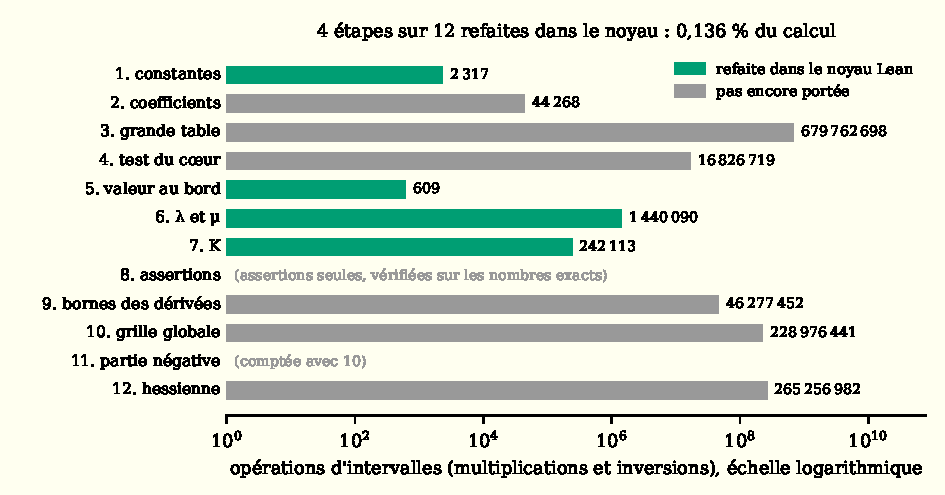
\includegraphics[width=\linewidth]{figures/c14_etapes}
\caption{Les douze étapes du certificat, par nombre d'opérations ; en vert, celles que le noyau Lean a refaites.}
\end{figure}
